
%%%%%%%%%%%%%%%%%%%%%%%%%%%%%%%%%%%%%%%%%%%%%%
\begin{figure*}[htb]
\centering
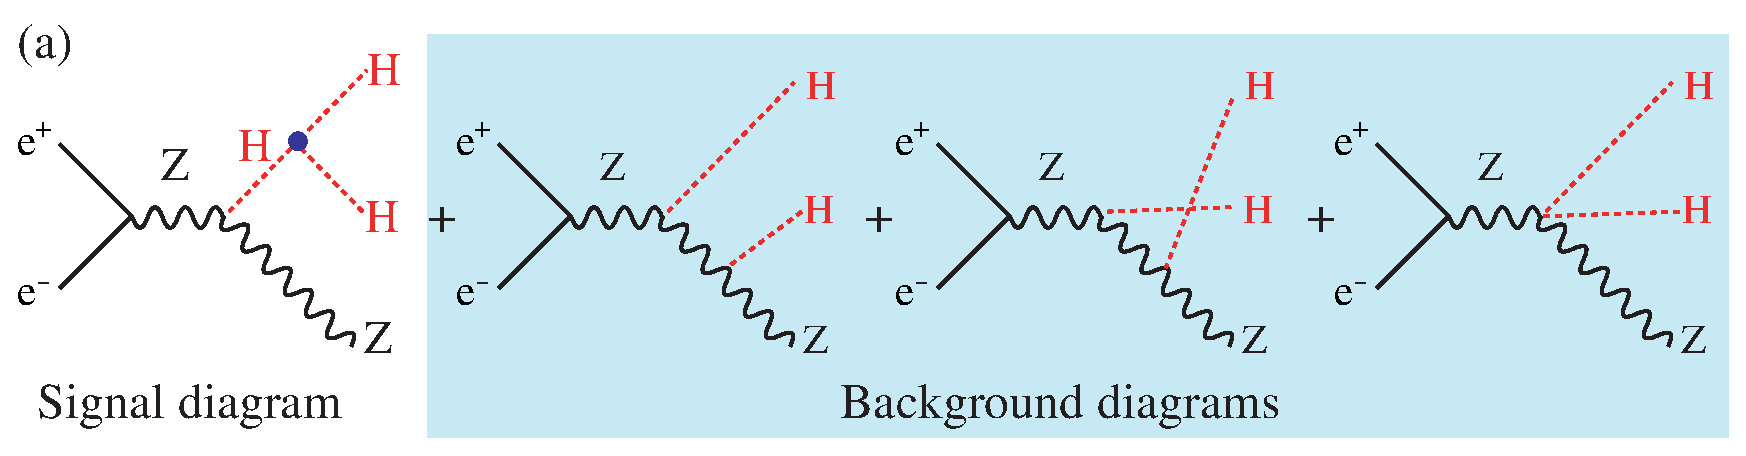
\includegraphics[width=130mm]{chapters/figures/zhhdiagrams.eps}
\\~\\
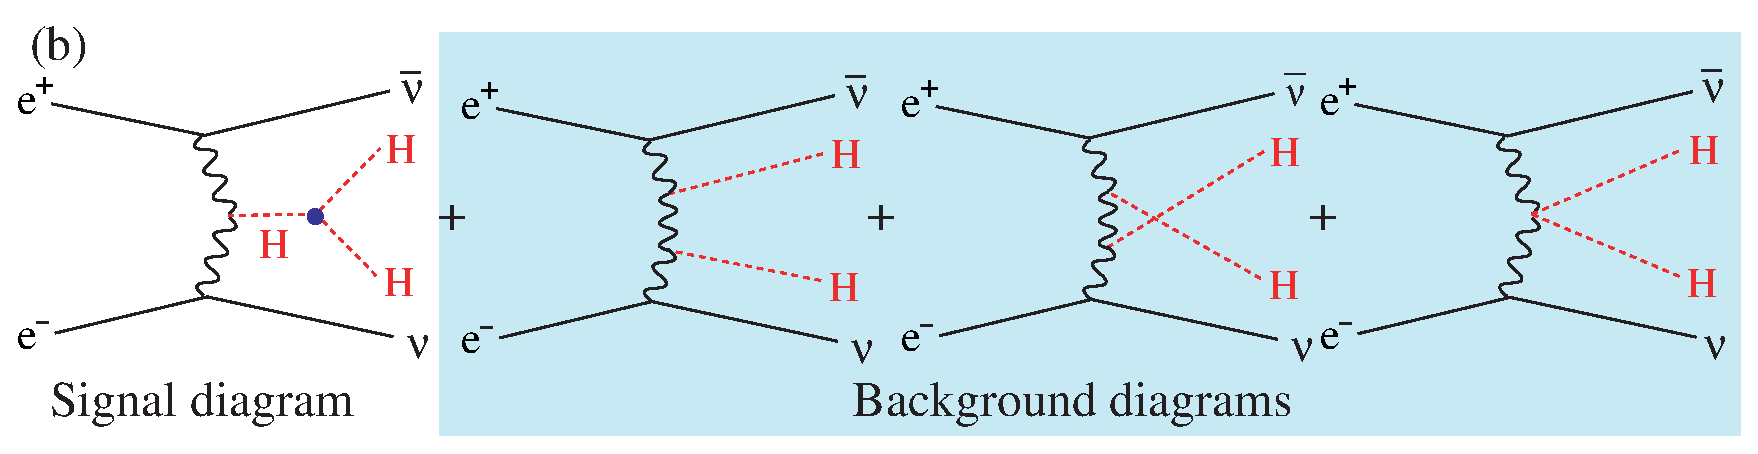
\includegraphics[width=130mm]{chapters/figures/vvhhdiagrams.eps}
\caption{Diagrams contributing to (a) $e^+e^- \to Zhh$ and (b) $e^+e^- \to \nu\bar{\nu}hh$.} 
\label{fig:hhdiagrams}
\end{figure*}
%%%%%%%%%%%%%%%%%%%%%%%%%%%%%%%%%%%%%%%%%%%%%%
%%%%%%%%%%%%%%%%%%%%%%%%%%%%%%%%%%%%%%%%%%%%%%
\begin{figure}[htb]
\centering
%\includegraphics[height=60mm]{01figs/xsec_HHprod_120.eps}
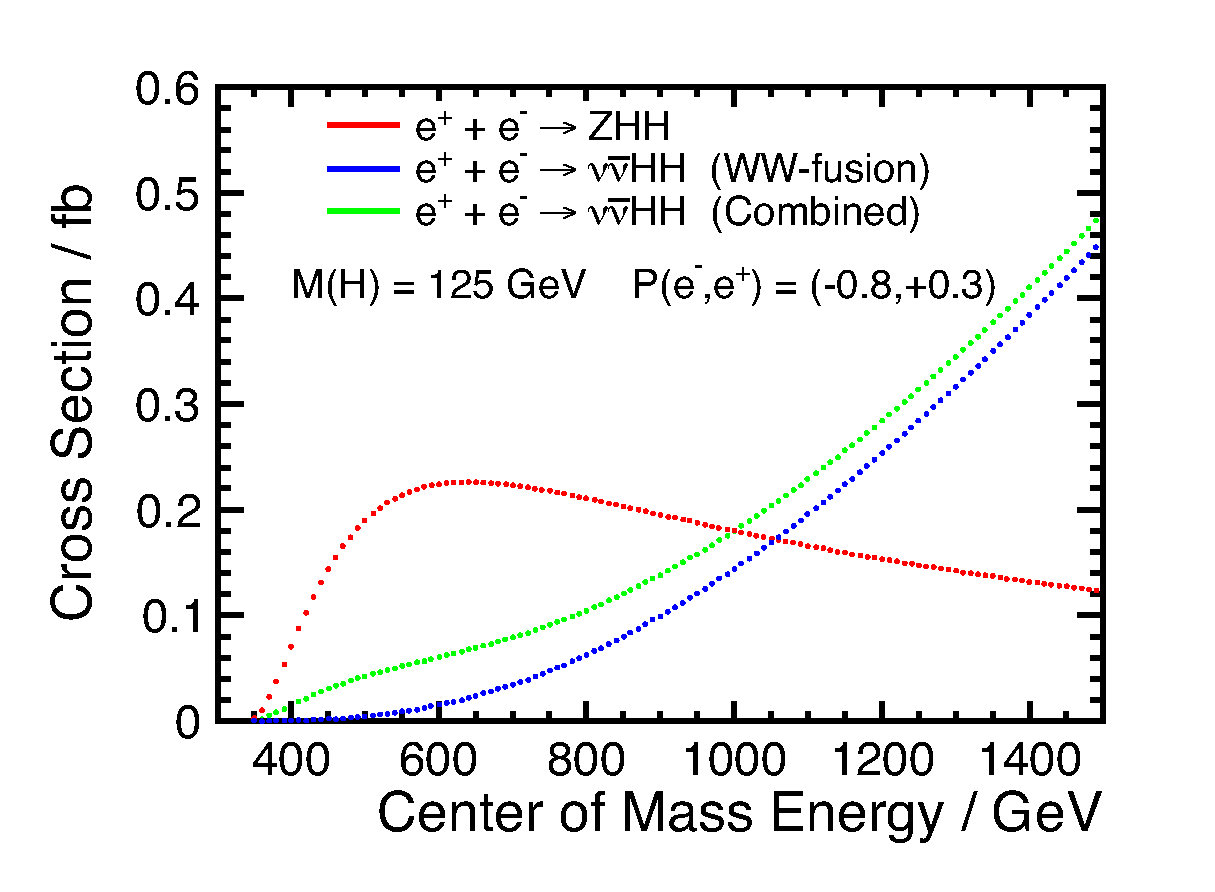
\includegraphics[width=0.85\hsize]{chapters/figures/HHXSec_l.eps}
\caption{Cross sections for the double Higgs production processes, 
$e^+e^- \to Zhh$ and $e^+e^- \to \nu\bar{\nu}hh$, as a function of $\sqrt{s}$ for $m_h=125\,$GeV.} 
\label{fig:sigzhh_vvhh}
\end{figure}
%%%%%%%%%%%%%%%%%%%%%%%%%%%%%%%%%%%%%%%%%%%%%%

\begin{figure*}[htb]
  \centering
  \begin{tabular}[c]{ccc}
    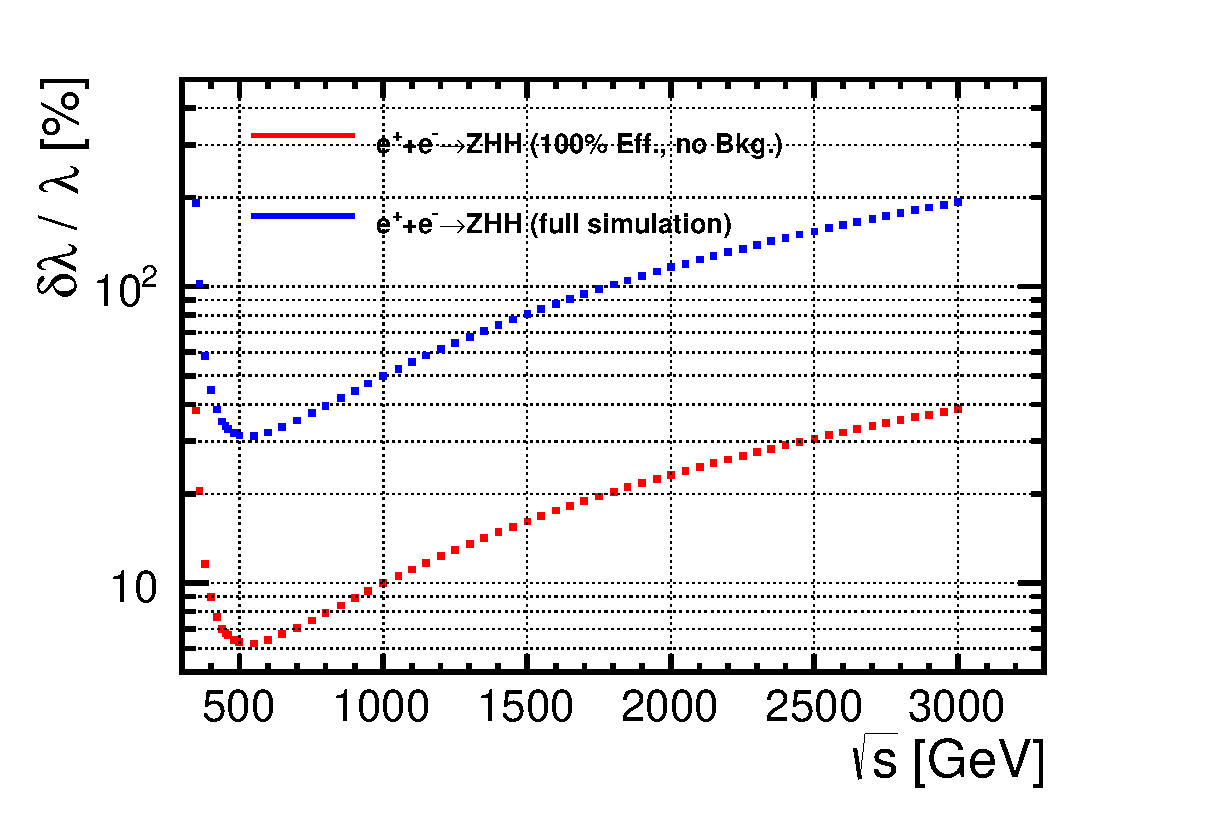
\includegraphics[width=0.45\hsize]{chapters/figures/coupling_zhh_125_-1.eps} &
    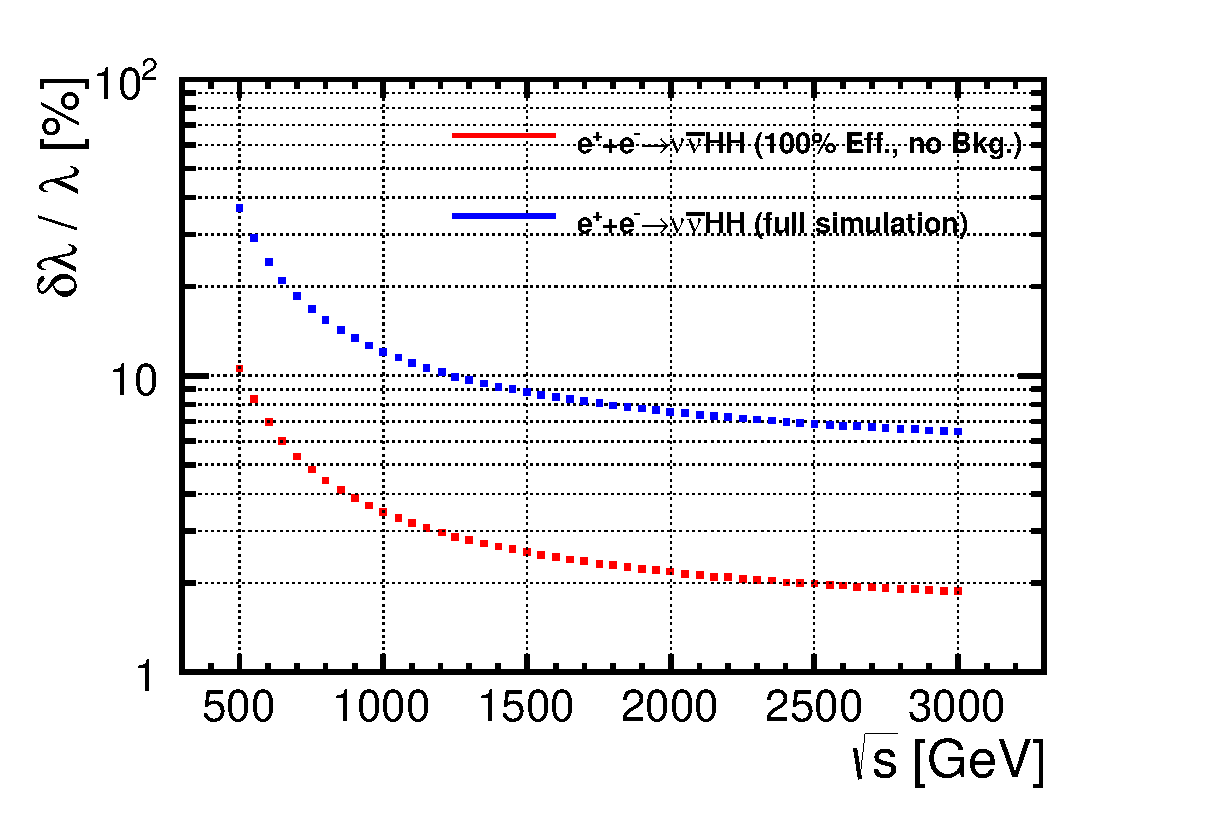
\includegraphics[width=0.45\hsize]{chapters/figures/coupling_nnhh_125_-1.eps} \\   
 \end{tabular}
  \caption{The expected precisions of $\lambda$ as a function of $\sqrt{s}$ for $e^+e^-\to Zhh$ ~(left) and
for $e^+e^-\to\nu\bar{\nu}hh$ ~(right). The two lines in each plot correspond to ideal situation (red) and 
realistic situation (blue) as described in the text. Same integrated luminosities of 4 $\mathrm{ab}^{-1}$ is 
assumed at all $\sqrt{s}$.}
  \label{fig:HHHSensitivity}
\end{figure*}

\begin{figure*}[htb]
  \centering
  \begin{tabular}[c]{ccc}
    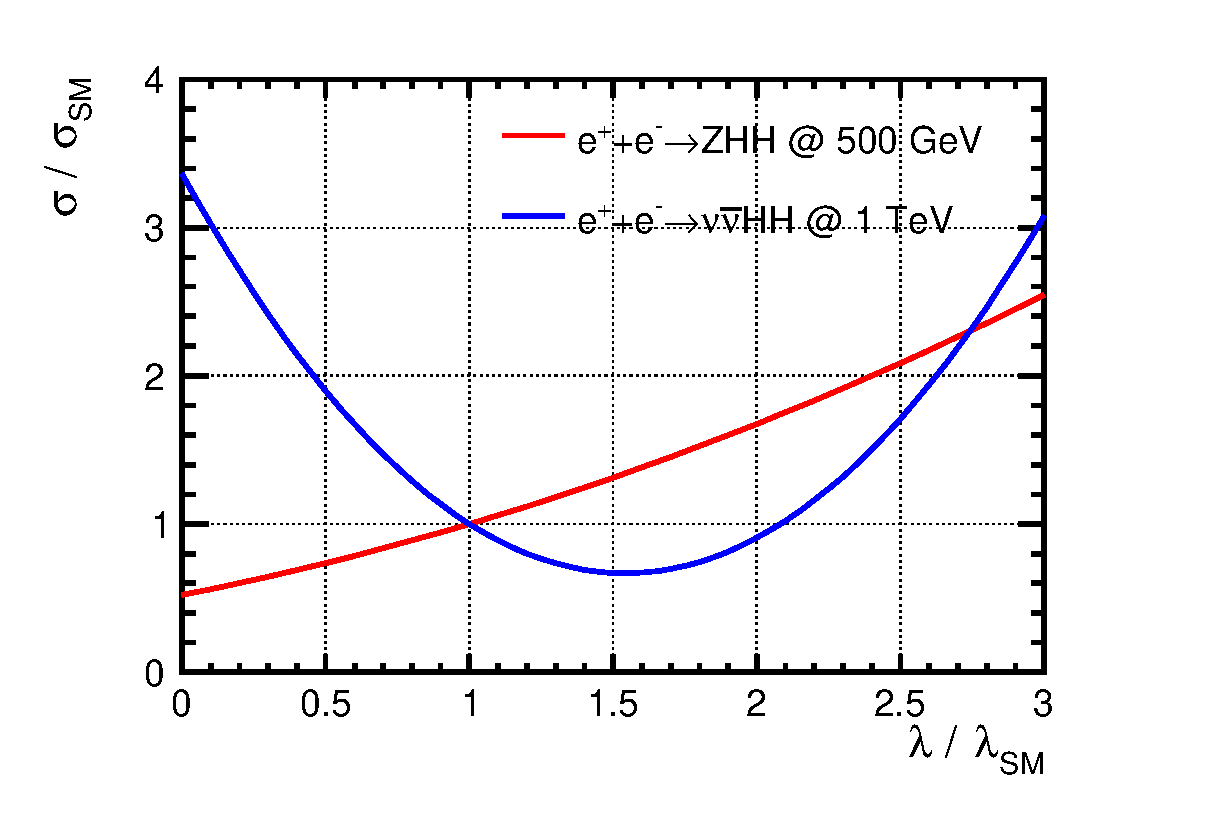
\includegraphics[width=0.45\hsize]{chapters/figures/xsec_coupling_BSM.eps} &
    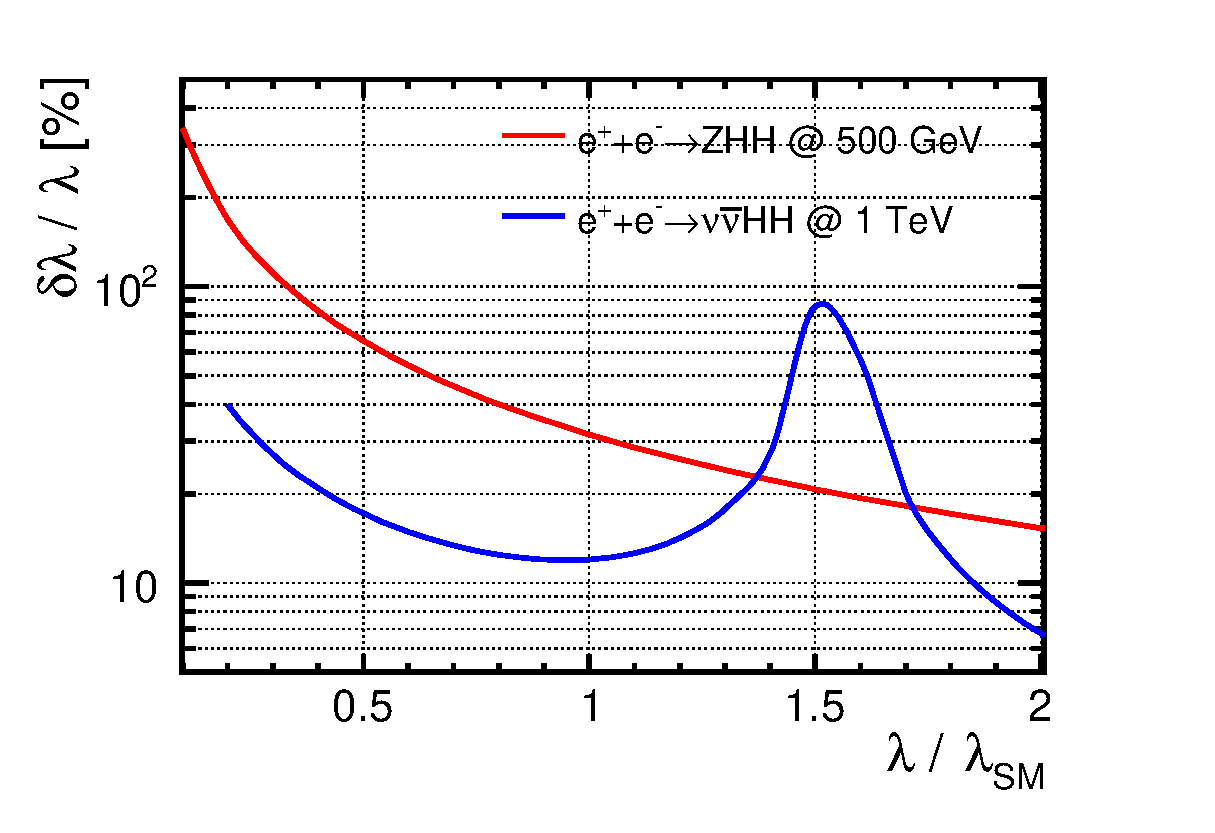
\includegraphics[width=0.45\hsize]{chapters/figures/precision_BSM_HHH.eps} \\   
 \end{tabular}
  \caption{Left: the cross section as a function of $\lambda$ for $e^+e^-\to Zhh$ ~(red line) and for 
  $e^+e^-\to\nu\bar{\nu}hh$ ~(blue line), where values of both $\lambda$ and $\sigma$ are scaled to their 
  SM values. Right: expected precisions of $\lambda$ when $\lambda$ is deviated from its SM value.}
  \label{fig:HHHBSM}
\end{figure*}

The  trilinear Higgs coupling can be measured at colliders in two
different ways. First, the coupling can be measured directly, using 
processes with Higgs pair production
that  diagrams involve the triple Higgs coupling at the tree level. 
Second, the coupling can be measured indirectly, since
radiative corrections to single-Higgs processes can include effects
due to the tripple Higgs coupling.

The important Higgs pair production reactions at $\ee$ colliders are 
$\ee\to ZHH$ and $\ee\to \nu\bar\nu HH$, shown in Fig.~\ref{fig:hhdiagrams}. 
Note in both reactions there are diagrams that do not involve trilinear Higgs coupling.
The first of these processes can be studied already at 500~GeV; 
the second, which is a 4-body process, requires somewhat higher energy. 
The cross sections of these two processes as a function of $\sqrt{s}$ are shown in Fig.~\ref{fig:sigzhh_vvhh}.
Full simulation studies at a $\sqrt{s}=$500~GeV show that a discovery of the
double Higgs-strahlung process is possible within the H20 program, 
using $Z\to l^+l^-/\nu\bar{\nu}/q\bar{q}$ and $hh\to b\bar{b}b\bar{b}/b\bar{b}WW^*$ channels.
With 4~\iab\ at 500~GeV, a combination of those decay channels
would yield a precision of 16.8\% on the total cross section for
$\ee\to ZHH$~\cite{Duerig:2016dvi,Tian:2013qmi,KurataHHH}.  Assuming the SM with only the
trilinear Higgs coupling free, this corresponds to an uncertainty of
27\% on that coupling.

At still higher energy vector boson fusion becomes the dominant
production channel. Making use of this channel, with  8~\iab\ at
1~TeV, the studies \cite{Tian:2013qmi,KurataHHH,Roloff:2019crr} show that, in the
same context of varying the trilinear Higgs coupling only, this
coupling can be determined to 10\%. 

The impact of the center-of-mass energies on the trilinear Higgs coupling
measurement is studied by extrapolating the full simulation results done 
at 500 GeV and 1 TeV to other energies. Due to the existence of diagrams 
that do not involve the trilinear Higgs coupling in both reactions, 
to get the correct extrapolation a careful 
analysis taking into account the dependence on $\sqrt{s}$ for both the
total cross sections and interference contributions was performed in \cite{TianHHH:2015}.
The results are shown in Fig.~\ref{fig:HHHSensitivity} as the blue lines for the two reactions. 
In addition to the results from realistic full simulations, the expectations for
the ideal case, that assumes no background and 100\% signal efficiency,
are also shown as the red lines. The differences between the blue and the read lines,
as large as a factor of 4-5, suggest that there might be huge room for improving
the realistic analysis in future. It can be concluded that $\sqrt{s}=500$-600 GeV is
optimal for $\ee\to Zhh$ and 1 TeV or above would be needed for $\ee\to\nu\bar{\nu}hh$. 

Since the trilinear Higgs coupling could be largely deviated from its SM value
in BSM models, in particular in electroweak baryogenesis models, 
it is interesting to see how the expected precisions would change.
Figure~\ref{fig:HHHBSM} gives the cross sections of the two reactions (left) and
the expected precisions of trilinear Higgs coupling (right),
as functions of the value of trilinear Higgs coupling. The natures of interferences in 
the two reactions are very different, constructive in $\ee\to Zhh$ while destructive 
in $\ee\to\nu\bar{\nu}hh$. Therefore it is important to note that 
the two reactions, useful at 500 GeV and 1 TeV
respectively, are complementary in determining the trilinear Higgs coupling. 
As an emphasis, if the trilinear Higgs coupling is indeed a factor of 2 larger in BSM,
the double Higgs-strahlung process at 500 GeV becomes very useful and 
would already provide 
a measurement of around 15\% precision for the trilinear Higgs coupling.

%%%[25]  J. Tian, LC-REP-2013-003, http://www-flc.desy.de/lcnotes/notes/LC-REP-2013-003.pdf
%%%[26]  M.   Kurata et  al,   LC-REP-2013-025,
%%%http://www-flc.desy.de/lcnotes/notes/LC-REP-2013-025.pdf


The indirect determination of the trilinear Higgs coupling is based on
the observation of McCullough~\cite{McCullough:2013rea} that the cross
section for $\ee\to ZH$ contains a radiative correction involving the
trilinear coupling that lower the cross section by about 1.5\% from
250~GeV to 500~GeV, with most of the decrease taking place below
350~GeV.  Taken a face value in the simple context with only the
trilinear coupling free, the ILC cross section measurements would determine the trilinear 
coupling to about 40\%.

It is important to note, however, that the determination of the
trilinear coupling involves two separate questions.  First, is the SM
violated?   The accuracies with which this question can be answered
are those given above.  Second, can the violation of the SM be
attributed to a change in the trilinear coupling or the Higgs
potential rather than being due to other possible new physics
effects?  A precise way to ask this question is: Can the shift of the
trilinear coupling be measured  independently of possible effects of
all 
other dimension-6 EFT operators?   To our knowledge, this latter
question has only been addressed for determinations of the trilinear
coupling at lepton colliders.   In Ref.~\cite{Barklow:2017awn} it is
shown that, after the ILC H20 program of single-Higgs measurements is
complete, the uncertainty in the measurement of the total cross
section for  $\ee\to ZHH$ receives a negligible 2.5\% uncertainty due
to variation of the other relevant dimension-6 EFT perturbations.   In
Ref.~\cite{DiVita:2017vrr}, it is shown that, when the cross section
for $\ee\to ZH$ is fit together with other relevant observables at
250~GeV and 500~GeV, the
uncertainty in the coupling is not substantially changed from the value of
40\%.  This study assumed perfect knowledge of precision electroweak observables, however;
the influence of current and projected electroweak constraints is under study. Assuming this result, the two
independent determinations of the trilinear couplings can be combined
into a determination of the trilinear coupling  with an accuracy of 23\% that is
also completely model-independent.  


